% The contents of this file is 
% Copyright (c) 2009-  Charles R. Severance, All Righs Reserved

\chapter{Using Web Services}

Once it became easy to retrieve documents and parse documents 
over HTTP using programs, it did not take long to develop 
an approach where we started producing documents that were specifically
designed to be consumed by other 
programs (i.e., not HTML to be displayed in a browser).

There are two common formats that we use when exchanging data across the web.
The ``eXtensible Markup Language'' or XML has been in use for a very long time 
and is best suited for exchanging document-style data.   When programs just want 
to exchange dictionaries, lists, or other internal information with each other,
they use JavaScript Object Notation or JSON (see \url{www.json.org}).  
We will look at both formats.

\section{eXtensible Markup Language - XML}

XML looks very similar to HTML, but XML is more structured 
than HTML.  Here is a sample of an XML document:

\beforeverb
\begin{verbatim}
<person>
  <name>Chuck</name>
  <phone type="intl">
     +1 734 303 4456
   </phone>
   <email hide="yes"/>
</person>
\end{verbatim}
\afterverb
%
Often it is helpful to think of an XML document as a tree structure
where there is a top tag {\tt person} and other tags such as {\tt phone}
are drawn as \emph{children} of their parent nodes.

\beforefig
\centerline{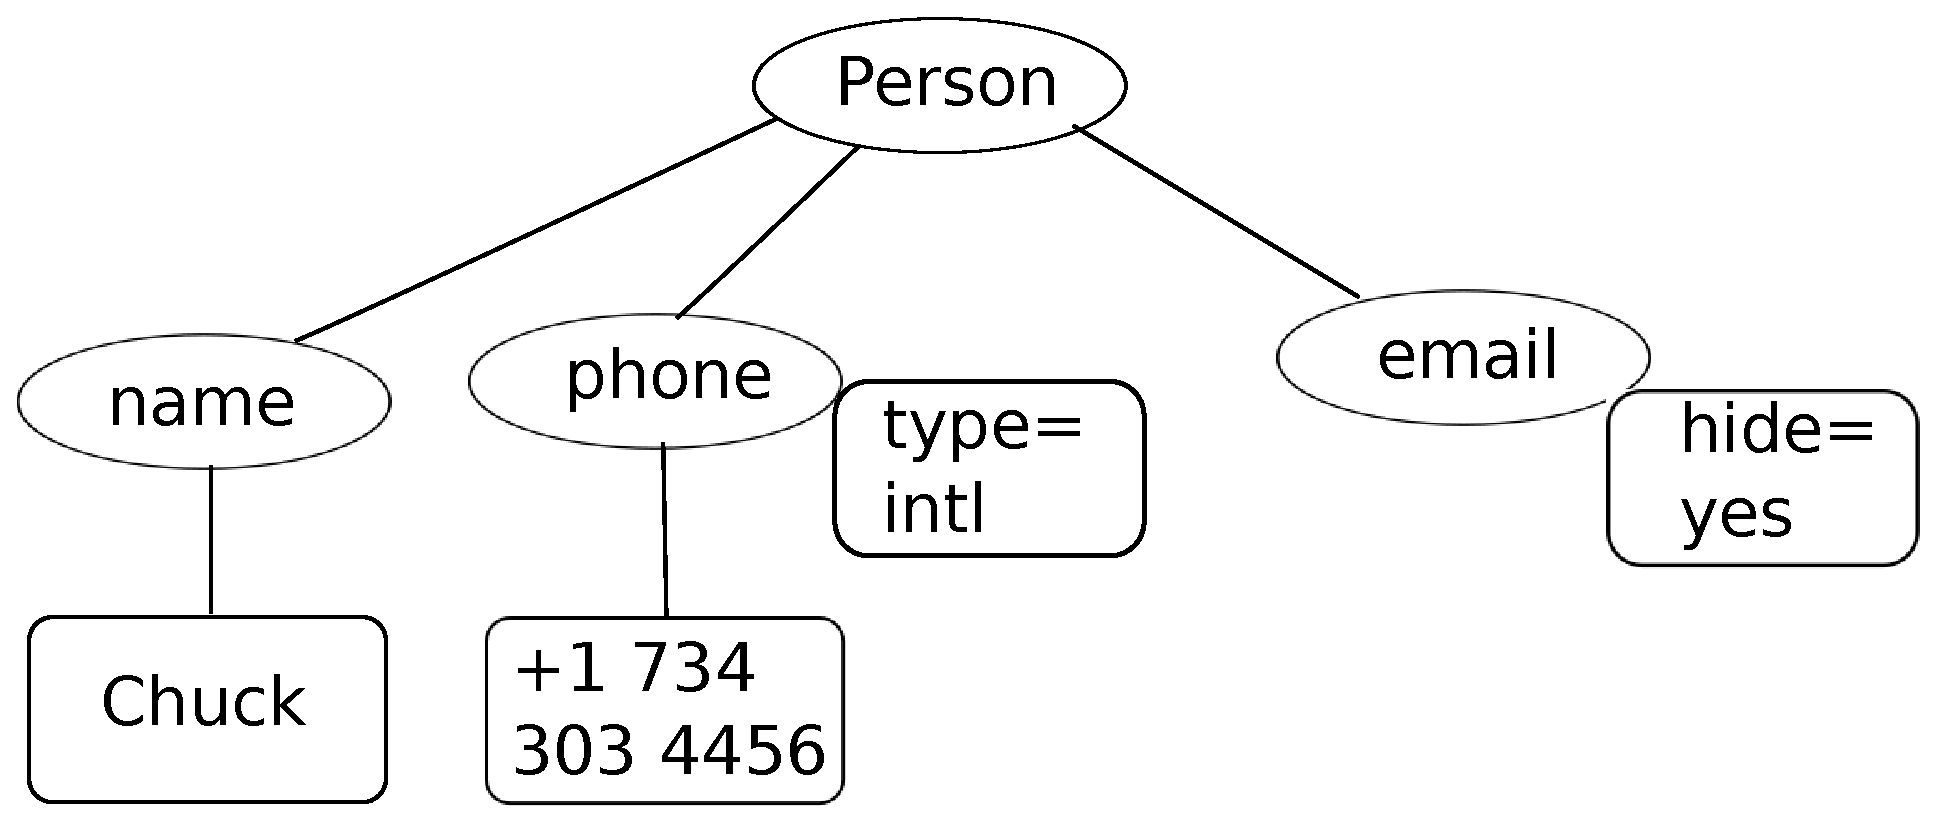
\includegraphics[height=1.50in]{figs2/xml-tree.eps}}
\afterfig

\section{Parsing XML}

\index{ElementTree}
\index{ElementTree!fromstring}
\index{ElementTree!find}
Here is a simple application that parses some XML
and extracts some data elements from the XML:

\beforeverb
\begin{verbatim}
import xml.etree.ElementTree as ET

data = '''
<person>
  <name>Chuck</name>
  <phone type="intl">
     +1 734 303 4456
   </phone>
   <email hide="yes"/>
</person>'''

tree = ET.fromstring(data)
print 'Name:',tree.find('name').text
print 'Attr:',tree.find('email').get('hide')
\end{verbatim}
\afterverb
%
Calling {\tt fromstring} converts the string representation
of the XML into a ``tree'' of XML nodes.  When the
XML is in a tree, we have a series of methods we can call to 
extract portions of data from the XML.  

The {\tt find} function searches through the 
XML tree and retrieves a {\bf node} that matches the specified tag.
Each node can have some text, some attributes (like hide), and
some ``child'' nodes.   Each node can be the top of a tree of nodes.

\beforeverb
\begin{verbatim}
Name: Chuck
Attr: yes
\end{verbatim}
\afterverb
%
Using an XML parser such as {\tt ElementTree} has the advantage
that while the XML in this example is quite simple, it turns
out there are many rules regarding valid XML and using 
{\tt ElementTree} allows us to extract data from XML without 
worrying about the rules of XML syntax.

\section{Looping through nodes}

\index{ElementTree!findall}
\index{ElementTree!get}
Often the XML has multiple nodes and we need to write a loop
to process all of the nodes.  In the following program, 
we loop through all of the {\tt user} nodes:

\beforeverb
\begin{verbatim}
import xml.etree.ElementTree as ET

input = '''
<stuff>
    <users>
        <user x="2">
            <id>001</id>
            <name>Chuck</name>
        </user>
        <user x="7">
            <id>009</id>
            <name>Brent</name>
        </user>
    </users>
</stuff>'''

stuff = ET.fromstring(input)
lst = stuff.findall('users/user')
print 'User count:', len(lst)

for item in lst:
    print 'Name', item.find('name').text
    print 'Id', item.find('id').text
    print 'Attribute', item.get('x')
\end{verbatim}
\afterverb
%
The {\tt findall} method retrieves a Python list of subtrees that
represent the {\tt user} structures in the XML tree.  Then we can 
write a {\tt for} loop that looks at each of the user nodes, and 
prints the {\tt name} and {\tt id} text elements as well as the 
{\tt x} attribute from the {\tt user} node.

\beforeverb
\begin{verbatim}
User count: 2
Name Chuck
Id 001
Attribute 2
Name Brent
Id 009
Attribute 7
\end{verbatim}
\afterverb
%

\section{JavaScript Object Notation - JSON}
\index{JSON}
\index{JavaScript Object Notation}

The JSON format was inspired by the object and array format used in the JavaScript
language.  But since Python was invented before JavaScript, Python's syntax
for dictionaries and lists influenced the syntax of JSON.  So the format of JSON
is nearly identical to a combination of Python lists and dictionaries.

Here is a JSON encoding that is roughly equivalent to the simple XML from above:

\beforeverb
\begin{verbatim}
{
  "name" : "Chuck",
  "phone" : {
    "type" : "intl",
    "number" : "+1 734 303 4456"
   },
   "email" : {
     "hide" : "yes"
   }
}
\end{verbatim}
\afterverb
%
You will notice some differences.  First, in XML, we can add attributes like
``intl'' to the ``phone'' tag.  In JSON, we simply have key-value pairs.  Also
the XML ``person'' tag is gone, replaced by a set of outer curly braces.  

In general, JSON structures are simpler than XML because JSON has fewer capabilities
than XML.  But JSON has the advantage that it maps {\em directly} to some combination
of dictionaries and lists.   And since nearly all programming languages 
have something equivalent to Python's dictionaries and lists, JSON is a very
natural format to have two cooperating programs exchange data.

JSON is quickly becoming the format of choice for nearly all data exchange between 
applications because of its relative simplicity compared to XML.

\section{Parsing JSON}

We construct our JSON by nesting dictionaries (objects) and lists as needed.  In 
this example, we represent a list of users where each user is a set of 
key-value pairs (i.e., a dictionary).  So we have a list of dictionaries.

In the following program, we use the built-in {\bf json} library to parse 
the JSON and read through the data.   Compare this closely to the equivalent
XML data and code above.  The JSON has less detail, so we must know in advance 
that we are getting a list and that the list is of users and each user is a
set of key-value pairs.  The JSON is more succinct (an advantage) but also is 
less self-describing (a disadvantage).

\beforeverb
\begin{verbatim}
import json

input = '''
[
  { "id" : "001",
    "x" : "2",
    "name" : "Chuck"
  } ,
  { "id" : "009",
    "x" : "7",
    "name" : "Brent"
  } 
]'''

info = json.loads(input)
print 'User count:', len(info)

for item in info:
    print 'Name', item['name']
    print 'Id', item['id']
    print 'Attribute', item['x']
\end{verbatim}
\afterverb
%

If you compare the code to extract data from the parsed JSON and XML
you will see that what we get from {\bf json.loads()} is a Python list
which we traverse with a {\tt for} loop, and each item within that list
is a Python dictionary.  Once the JSON has been parsed, we can use the Python
index operator to extract the various bits of data for each user.  We don't
have to use the JSON library to dig through the parsed JSON, since the returned
data is simply native Python structures.

The output of this program is exactly the same as the XML version above.

\beforeverb
\begin{verbatim}
User count: 2
Name Chuck
Id 001
Attribute 2
Name Brent
Id 009
Attribute 7
\end{verbatim}
\afterverb
%
In general, there is an industry trend away from XML and towards JSON for 
web services.  Because the JSON is simpler and more directly maps to native 
data structures we already have in programming languages, the parsing 
and data extraction code is usually simpler and more direct when using JSON.
But XML is more self-descriptive than JSON and so there are 
some applications where XML retains an advantage.  For example, most word 
processors store documents internally using XML rather than JSON.

\section{Application Programming Interfaces}

We now have the ability to exchange data between applications using HyperText
Transport Protocol (HTTP) and a way to represent complex data that we are 
sending back and forth between these applications using eXtensible 
Markup Language (XML) or JavaScript Object Notation (JSON).

The next step is to begin to define and document ``contracts'' between 
applications using these techniques. The general name for these 
application-to-application contracts is {\bf Application Program 
Interfaces} or APIs.  When we use an API, generally one program
makes a set of {\bf services} available for use by other applications
and publishes the APIs (i.e., the ``rules'') that must be followed to 
access the services provided by the program.

When we begin to build our programs where the functionality of
our program includes access to services provided by other programs, 
we call the approach a {\bf Service-Oriented Architecture} or SOA.
A SOA approach is one where our overall application makes use of 
the services of other applications.  A non-SOA approach is where the
application is a single standalone application which contains all of the
code necessary to implement the application.

We see many examples of SOA when we use the web.  We can go to a single 
web site and book air travel, hotels, and automobiles all from a 
single site.  The data for hotels is not stored on the airline computers. 
Instead, the airline computers contact the services on the hotel computers
and retrieve the hotel data and present it to the user.  When the user
agrees to make a hotel reservation using the airline site, the airline site uses
another web service on the hotel systems to actually make the reservation.
And when it comes time to charge your credit card for the whole transaction, 
still other computers become involved in the process.

\beforefig
\centerline{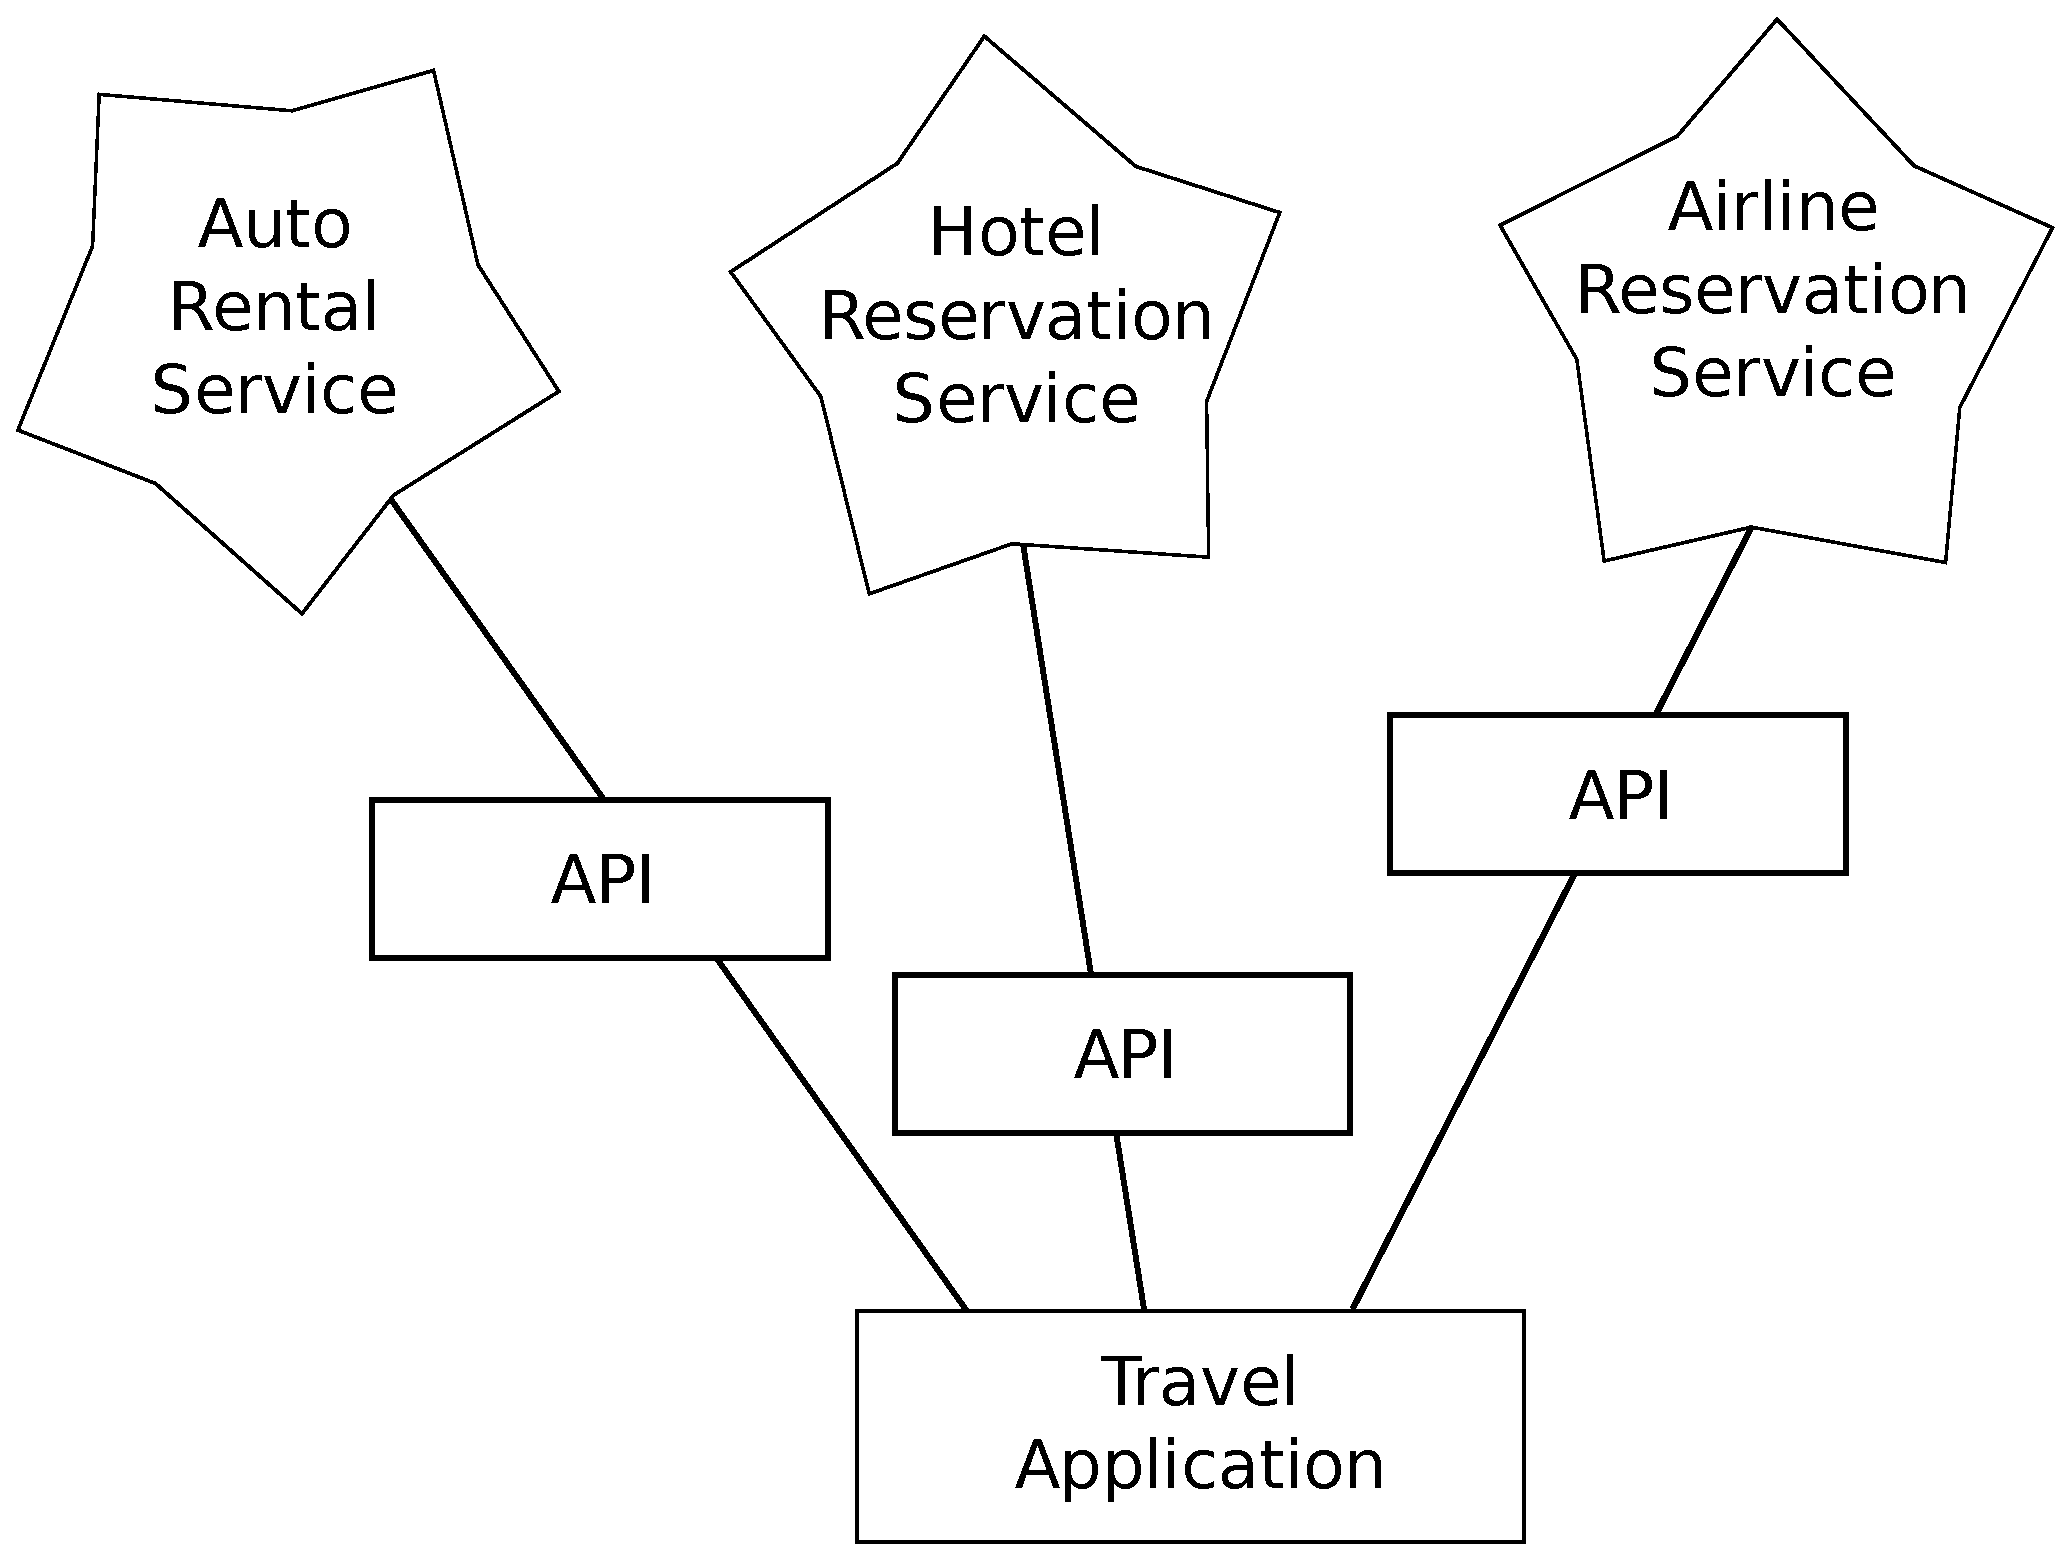
\includegraphics[height=2.50in]{figs2/soa.eps}}
\afterfig

A Service-Oriented Architecture has many advantages including: (1) we 
always maintain only one copy of data (this is particularly important
for things like hotel reservations where we do not want to over-commit)
and (2) the owners of the data can set the rules about the use of their 
data.   With these advantages, an SOA system must be carefully designed
to have good performance and meet the user's needs.

When an application makes a set of services in its API available over the web, 
we call these {\bf web services}. 

\section{Google geocoding web service}
\index{Google}
\index{geocoding}
\index{web service}

Google has an excellent web service that allows us to make use of their 
large database of geographic information.   We can submit a geographical
search string like ``Ann Arbor, MI'' to their geocoding API and have Google 
return its best guess as to where on a map we might find our search string and
tell us about the landmarks nearby.

The geocoding service is free but rate limited so you cannot make unlimited
use of the API in a commercial application.   But if you have some survey data
where an end user has entered a location in a free-format input box, you can use
this API to clean up your data quite nicely.  

{\em When you are using a free API like Google's geocoding API, you need
to be respectful in your use of these resources.  If too many people abuse the
service, Google might drop or significantly curtail its free service.}
\index{rate limiting}

You can read the online documentation for this service, but it is quite simple
and you can even test it using a browser by typing the following URL into your 
browser:

\url{http://maps.googleapis.com/maps/api/geocode/json?sensor=false &address=Ann+Arbor%2C+MI}

Make sure to unwrap the URL and remove any spaces from the URL before pasting
it into your browser.

The following is a simple application to prompt the user for a search string,
call the Google geocoding API, and extract information from the returned JSON.

\beforeverb
\begin{verbatim}
import urllib
import json

serviceurl = 'http://maps.googleapis.com/maps/api/geocode/json?'

while True:
    address = raw_input('Enter location: ')
    if len(address) < 1 : break

    url = serviceurl + urllib.urlencode({'sensor':'false', 
          'address': address})
    print 'Retrieving', url
    uh = urllib.urlopen(url)
    data = uh.read()
    print 'Retrieved',len(data),'characters'

    try: js = json.loads(str(data))
    except: js = None
    if 'status' not in js or js['status'] != 'OK':
        print '==== Failure To Retrieve ===='
        print data
        continue

    print json.dumps(js, indent=4)

    lat = js["results"][0]["geometry"]["location"]["lat"]
    lng = js["results"][0]["geometry"]["location"]["lng"]
    print 'lat',lat,'lng',lng
    location = js['results'][0]['formatted_address']
    print location
\end{verbatim}
\afterverb
%
The program takes the search string and constructs a URL with the
search string as a properly encoded parameter and then uses
{\bf urllib} to retrieve the text from the Google geocoding API.
Unlike a fixed web page, the data we get depends on the parameters
we send and the geographical data stored in Google's servers.

Once we retrieve the JSON data, we parse it with the {\bf json}
library and do a few checks to make sure that we received good data, 
then extract the information that we are looking for.

The output of the program is as follows (some of the returned
JSON has been removed):

\beforeverb
\begin{verbatim}
$ python geojson.py
Enter location: Ann Arbor, MI
Retrieving http://maps.googleapis.com/maps/api/
  geocode/json?sensor=false&address=Ann+Arbor%2C+MI
Retrieved 1669 characters
{
    "status": "OK", 
    "results": [
        {
            "geometry": {
                "location_type": "APPROXIMATE", 
                "location": {
                    "lat": 42.2808256, 
                    "lng": -83.7430378
                }
            }, 
            "address_components": [
                {
                    "long_name": "Ann Arbor", 
                    "types": [
                        "locality", 
                        "political"
                    ], 
                    "short_name": "Ann Arbor"
                } 
            ], 
            "formatted_address": "Ann Arbor, MI, USA", 
            "types": [
                "locality", 
                "political"
            ]
        }
    ]
}
lat 42.2808256 lng -83.7430378
Ann Arbor, MI, USA
Enter location:
\end{verbatim}
\afterverb
%
You can download 
\url{www.py4inf.com/code/geojson.py} and 
\url{www.py4inf.com/code/geoxml.py} to explore the JSON
and XML variants of the Google geocoding API. 

\section{Security and API usage}
\index{OAuth}
\index{API!key}

It is quite common that you need some kind of 
``API key'' to make use of a vendor's API.  The
general idea is that they want to know who is using 
their services and how much each user is using.  
Perhaps they have free and pay tiers of their services
or have a policy that limits the number of requests 
that a single individual can make during a particular 
time period.

Sometimes once you get your API key, you simply include
the key as part of POST data or perhaps as a parameter
on the URL when calling the API.

Other times, the vendor wants increased assurance of
the source of the requests and so they add expect you 
to send cryptographically signed messages using shared
keys and secrets.   A very common technology that is used 
to sign requests over the Internet is called {\bf OAuth}.
You can read more about the OAuth protocol at
\url{http://www.oauth.net}.

As the Twitter API became increasingly valuable, Twitter
went from an open and public API to an API that required
the use of OAuth signatures on each API request. Thankfully
there are still a number of convenient and free OAuth libraries
so you can avoid writing an OAuth implementation from scratch
by reading the specification.  These libraries are of 
varying complexity and have varying degrees of
richness.  The OAuth web site has information about various 
OAuth libraries.

For this next sample program we will download the files 
{\bf twurl.py}, {\bf hidden.py}, 
{\bf oauth.py}, 
and
{\bf twitter1.py} from 
\url{www.py4inf.com/code} and put them all in a folder
on your computer.

To make use of these programs you will need to have a Twitter
account, and authorize your Python code as an application,
set up a key, secret, token and token secret.  You will edit
the file {\bf hidden.py} and put these four strings into the
appropriate variables in the file:

\beforeverb
\begin{verbatim}
    def auth() :
        return { "consumer_key" : "h7L...GNg",
            "consumer_secret" : "dNK...7Q",
            "token_key" : "101...GI",
            "token_secret" : "H0yM...Bo" }
\end{verbatim}
\afterverb
%
The Twitter web service are accessed using a URL like this:

\url{https://api.twitter.com/1.1/statuses/user_timeline.json}

But once all of the security information has been added, the URL
will look more like:

\beforeverb
\begin{verbatim}
https://api.twitter.com/1.1/statuses/user_timeline.json?count=2
&oauth_version=1.0&oauth_token=101...SGI&screen_name=drchuck
&oauth_nonce=09239679&oauth_timestamp=1380395644
&oauth_signature=rLK...BoD&oauth_consumer_key=h7Lu...GNg
&oauth_signature_method=HMAC-SHA1
\end{verbatim}
\afterverb
%
You can read the OAuth specification if you want to
know more about the meaning of the various parameters that
are added to meet the security requirements of OAuth.  

For the programs we run with Twitter, we hide all the 
complexity in the files {\bf oauth.py} and {\bf twurl.py}.
We simply set the secrets in {\bf hidden.py} and then 
send the desired URL to the {\bf twurl.augment()} 
function and the library code adds all the necessary 
parameters to the URL for us.

This program ({\bf twitter1.py}) retrieves the timeline
for a particular Twitter user and returns it to us in JSON
format in a string.  We simply print the first 250 characters
of the string:

\beforeverb
\begin{verbatim}
import urllib
import twurl

TWITTER_URL='https://api.twitter.com/1.1/statuses/user_timeline.json'

while True:
    print ''
    acct = raw_input('Enter Twitter Account:')
    if ( len(acct) < 1 ) : break
    url = twurl.augment(TWITTER_URL,
        {'screen_name': acct, 'count': '2'} )
    print 'Retrieving', url
    connection = urllib.urlopen(url)
    data = connection.read()
    print data[:250]
    headers = connection.info().dict
    # print headers
    print 'Remaining', headers['x-rate-limit-remaining']
\end{verbatim}
\afterverb
%
When the program runs it produces the following output: 
 
\beforeverb
\begin{verbatim}
Enter Twitter Account:drchuck
Retrieving https://api.twitter.com/1.1/ ...
[{"created_at":"Sat Sep 28 17:30:25 +0000 2013","
id":384007200990982144,"id_str":"384007200990982144",
"text":"RT @fixpert: See how the Dutch handle traffic 
intersections: http:\/\/t.co\/tIiVWtEhj4\n#brilliant",
"source":"web","truncated":false,"in_rep
Remaining 178

Enter Twitter Account:fixpert
Retrieving https://api.twitter.com/1.1/ ...
[{"created_at":"Sat Sep 28 18:03:56 +0000 2013",
"id":384015634108919808,"id_str":"384015634108919808",
"text":"3 months after my freak bocce ball accident, 
my wedding ring fits again! :)\n\nhttps:\/\/t.co\/2XmHPx7kgX",
"source":"web","truncated":false,
Remaining 177

Enter Twitter Account:
\end{verbatim}
\afterverb
%
Along with the returned timeline data, Twitter also returns
metadata about the request in the HTTP response headers. 
One header in particular, {\bf x-rate-limit-remaining}, informs
us how many more requests we can make before we will be shut 
off for a short time period.  You can see that our remaining 
retrievals drop by one each time we make a request to the 
API.

In the following example, we retrieve a user's Twitter friends,
parse the returned JSON, and extract some of the information
about the friends.  We also dump the JSON after parsing and
``pretty-print'' it with an indent of four characters to allow
us to pore through the data when we want to extract more fields.

\beforeverb
\begin{verbatim}
import urllib
import twurl
import json

TWITTER_URL = 'https://api.twitter.com/1.1/friends/list.json'

while True:
    print ''
    acct = raw_input('Enter Twitter Account:')
    if ( len(acct) < 1 ) : break
    url = twurl.augment(TWITTER_URL,
        {'screen_name': acct, 'count': '5'} )
    print 'Retrieving', url
    connection = urllib.urlopen(url)
    data = connection.read()
    headers = connection.info().dict
    print 'Remaining', headers['x-rate-limit-remaining']
    js = json.loads(data)
    print json.dumps(js, indent=4)

    for u in js['users'] :
        print u['screen_name']
        s = u['status']['text']
        print '  ',s[:50]
\end{verbatim}
\afterverb
%
Since the JSON becomes a set of nested Python lists and dictionaries,
we can use a combination of the index operation and {\tt for} loops to 
wander through the returned data structures with very little 
Python code.

The output of the program looks as follows (some of the data items 
are shortened to fit on the page):

\beforeverb
\begin{verbatim}
Enter Twitter Account:drchuck
Retrieving https://api.twitter.com/1.1/friends ...
Remaining 14
{
    "next_cursor": 1444171224491980205, 
    "users": [
        {
            "id": 662433, 
            "followers_count": 28725, 
            "status": {
                "text": "@jazzychad I just bought one .__.", 
                "created_at": "Fri Sep 20 08:36:34 +0000 2013", 
                "retweeted": false, 
            }, 
            "location": "San Francisco, California", 
            "screen_name": "leahculver", 
            "name": "Leah Culver", 
        }, 
        {
            "id": 40426722, 
            "followers_count": 2635, 
            "status": {
                "text": "RT @WSJ: Big employers like Google ...", 
                "created_at": "Sat Sep 28 19:36:37 +0000 2013", 
            }, 
            "location": "Victoria Canada", 
            "screen_name": "_valeriei", 
            "name": "Valerie Irvine", 
    ], 
    "next_cursor_str": "1444171224491980205"
}
leahculver
   @jazzychad I just bought one .__.
_valeriei
   RT @WSJ: Big employers like Google, AT&amp;T are h
ericbollens
   RT @lukew: sneak peek: my LONG take on the good &a
halherzog
   Learning Objects is 10. We had a cake with the LO,
scweeker
   @DeviceLabDC love it! Now where so I get that "etc

Enter Twitter Account:
\end{verbatim}
\afterverb
%
The last bit of the output is where we see the for loop reading the
five most recent ``friends'' of the {\bf drchuck} Twitter account 
and printing the most recent status for each friend. There is a 
great deal more data available in the returned JSON.  If you look
in the output of the program, you can also see that the ``find the friends''
of a particular account has a different rate limitation than 
the number of timeline queries we are allowed to run per time period.

These secure API keys allow Twitter to have solid confidence that they 
know who is using their API and data and at what level.   The 
rate-limiting approach allows us to do simple, personal data retrievals but
does not allow us to build a product that pulls data from their API 
millions of times per day.

\section{Glossary}

\begin{description}

\item[API:] Application Program Interface - A contract between
applications that defines the patterns of interaction between 
two application components.
\index{API}

\item[ElementTree:] A built-in Python library used to parse XML data.
\index{ElementTree}

\item[JSON:] JavaScript Object Notation. A format that allows for 
the markup of structured data based on the syntax of JavaScript
Objects.
\index{JSON}
\index{JavaScript Object Notation}

\item[SOA:] Service-Oriented Architecture. When an application is 
made of components connected across a network.
\index{SOA}
\index{Service Oriented Architecture}

\item[XML:] eXtensible Markup Language. A format that allows for 
the markup of structured data.
\index{XML}
\index{eXtensible Markup Language}

\end{description}

\section{Exercises}

\begin{ex}
Change either the 
\url{www.py4inf.com/code/geojson.py} or
\url{www.py4inf.com/code/geoxml.py} to print out the 
two-character country code from the retrieved data.
Add error checking so your program does not traceback
if the country code is not there.  Once you have it 
working, search for ``Atlantic Ocean'' and make sure
it can handle locations that are not in any country.
\end{ex}

